\section{Introduction}
A common challenge in the design of semiconductor technologies is the sensitivity of electronics to cosmic radiation. This phenomenon is becoming increasingly apparent as technologies scale toward smaller feature sizes, altering the functionality of modern processors and FPGAs. This is particularly critical in safety domains such as automotive systems and space exploration, where even a single undetected error can lead to catastrophic failure, data corruption, or loss of mission objectives.

Specifically, ionizing radiation from cosmic rays can alter information stored in transistors. As a charged particle traverses a memory cell, it can deposit sufficient charge to invert a bit's logical state. This phenomenon is known as a \textit{bit-flip} error. Figure \ref{fig:radiation} illustrates this behavior.

\begin{figure}[htbp]
    \centering
    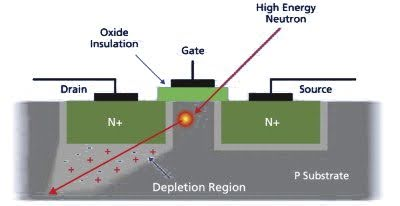
\includegraphics[width=1\linewidth]{assets/bitflip.jpg}
    \caption{Bit Altering Caused by Cosmic Rays}
    \label{fig:radiation}
\end{figure}

These faults fall into two categories, a \textit{Single Event Upset (SEU)}, where a single bit is altered in a device's memory, and \textit{Multiple-Bit Upsets (MBU)}, where several adjacent bits are corrupted simultaneously. \textit{MBUs} have become increasingly prevalent as technology is evolving and memory is becoming more dense.\\

Ensuring system reliability under such conditions requires more than theoretical fault models or post-deployment observation. Instead, engineers must proactively evaluate system behavior under similar fault conditions during the design and validation process. For this reason, fault injection has emerged as a key engineering methodology, by introducing actual faults into a system in order to observe and test its response, with the goal of designing fault tolerance mechanisms.\\

Fault Injection approaches can be broadly classified into three categories:
\begin{enumerate}
    \item \textbf{Hardware-based techniques:} Using physical equipment (e.g., radiation sources or pin injection) to alter device states.
    \item \textbf{Software-Implemented Fault Injection (SWIFI):} Using software routines to corrupt memory or registers at the operating system or application level.
    \item \textbf{Simulation and Emulation:} Utilizing Instruction Set Architecture (ISA) simulators or Register Transfer Level (RTL) models to inject faults into virtual hardware descriptions, enabling early analysis of both reliability and resource utilization without physical prototypes.
\end{enumerate}